\chapter{History and recent advancements}
\label{kap:kap1}

The size of information and data grows exponentially over years. In order to store this data, we use different data structures. These data structures not only represent the data but also enable us to make certain operations over them. There is a significant effort in not only speeding up these structures but also making them smaller in size so that they can be managed in memory and not on a secondary data storage thas is often orders of magnitude times slower. The key factor is to find the right balance between the speed of common operations and the amount of information that we need to store. These data structures often find usage in bioinformatics and compression algorithms.

\section{Space-efficient data structures}

When we measure how space-efficient the data structure is, we often measure this in size of additional information that we store alongside the original data. Most of the time, with the complexity of operations that our data structure supports, the size of helper data stored alongside the original data also increases. The original data can be also compressed to further increase the space-efficiency. To remove ambiguity, it is common to measure the size of the original data in the information-theoretical optimal number of bits used to store the original data. Over years, it was needed to further divide space-efficient data structures to distinguish between several types of efficiency. We will now introduce the basic definition that distinguishes between space-efficiency of data structures and is now widely used:

\begin{theorem}
Let $X$ denote the information-theoretical optimal number of bits needed to store the data. A data structure representing this data is called:
\begin{itemize}
    \item compact if it takes $O(X)$ bits of space
    \item succinct if it takes $X + o(X)$ bits of space
    \item implicit if it takes $X + O(1)$ bits of space
\end{itemize}
\end{theorem}

As an example, the common representation of the sequence of characters - string - in a common programming language such as C uses the null-termination method. This method stores the original string unchanged in memory with the special null termination character just after the end of the string denoting the end of the string. It is easy to see that this representation is implicit as it only stores a constant number of additional characters. To represent the string, we could also store the string and only remember it's length, not using the null termination character. This would, however, lead to a succinct data structure as we need $O(log(X))$ bits to store the length of the string.

The amount of data that these types of structures are dealing with is many times too big to store a linear number of additional data. In our work, we will focus on solutions and most of the work in the area that aims at a sublinear number of additional stored data.

We should also note, that the additional requirement on the data structure to be space-efficient many times leads to worse time complexity. Even if the theoretical time complexity remains the same for compressed data structures, the real-world implementation can suffer in performance as the methods that are used to work with compressed data are many times not ideal in the classical computer model.

\subsection{K-th order entropy}

\begin{theorem}
Let $S$ be a string of size $n$ and $n_i$ denoting number of occurences of character
$i$. Empirical entropy of the string $S$ is denoted $H_0(S)$ and defined as:
\begin{center}
$H_0(S) = \frac{1}{n} \sum_{i \in [1, \sigma]} \frac{n_i}{n}\cdot log(\frac{n}{n_i})$
\end{center}
\end{theorem}

Most of these algorithms use also as a measure of information stored a $k$-order empirical entropy.

\begin{theorem}
Let $S$ be a string of size $n$ and construct $T_A$ as a string of symbols following $k$-tuple ($k \geq 1$) $A$ in $S$.
$k$-order empirical entropy of $S$ denoted $H_k(S)$ is defined as:
\begin{center}
$H_k(S) = \frac{1}{n} \sum_{A \in [1, \sigma ]^k} |T_A| H_0(T_A)$
\end{center}
\end{theorem}

We can think of the $k$-order empirical entropy as a measure of information that is emitted with respect to the previous $k$-characters. This type of measure is especially useful when we know that we are dealing with some data where the symbol is somehow dependent on previously emitted symbols. This kind of behaviour can be seen for example in the sequences of characters from natural languages.

\section{History and recent progress in the field}

We will now look briefly into the history and then on the most recent results in this topic. The field dates back to the Jacobsen work on static succinct data structures \cite{jacobson1988succinct}. Jacobsen distinguishes between data compression when we take the big chunk of data and try to fit it into a smaller place and
data optimization when we want to actively do queries over this stored information. His work mainly looked into a space-efficient representation of linked lists, trees and direct-acyclic graphs with ability to do traversing over them.

There are of course many possible data structures and operations that they can support in order to be reasonable to use. We will now look at the most common operations that are supported in the succinct data structures. From our observations, the most basic operations used are $rank$ and $select$.

\begin{theorem}
Lets $N$ be a finite sequence of $n$ elements.
We define two operations rank and select: \\
$rank_q(x) = | \{k; k \in [ 1, 2, \ldots, x] : N[k] = q  \} |$ \\
$select_q(x) = min \{k; k \in [ 1, 2, \ldots, n) : rank_q(k)=x  \} $
\end{theorem}

In other words, $rank_q(x)$ denotes the number of elements in $N$ that are equal to $q$ and their position in $N$ is less than $x$. $select_q(x)$ returns the position of $x$-th occurence of $q$. We will later show, why these two operations are useful.

\subsection{Bit-vector}

One of the most basic data structures used as a building block in many other succinct data structures is bit-vector.

\begin{theorem}
Let $B$ be a sequence of $n$ elements from the alphabet $\Sigma = \{0, 1\}$. We call a bit-vector data structure storing this sequence
and allowing operation $access(i)$ that returns the $i$-th character.
\end{theorem}

When looking at the space-efficient implementation of a bit-vector we need to see that as we have only symbols 0 and 1 of length 1 we are not able to compress bit-vector by using some other codes for this values. The one way to compress the bit-vector is groups more of the symbols and trying to represent somehow this new block. We will now show some basic techniques to represent and compress the bit-vectors. 

\subsection{RRR}

RRR is common method used for representing static bitmaps introduced by Raman, Raman, Rao \cite{raman2007succinct} achieving space complexity $nH_0(S) + O(log(n))$. We split the binary representation of data into big chunks, which we call blocks.
Each $f$ of subsequent blocks are connected into non-overlapping superblocks. Each block is then encoded as a pair of integers $(c, o)$. $c$
is the count of the set bits in the corresponding block and $o$ is an offset into the table $T[c]$ that stores in lexicographic order all the sequences of
length $b$ with $c$ bits set to 1.

\subsection{Run length encoding}

Another widely used type of storage is run-length encoding. We will assume, that one of the values in bit-vector(either 0 or 1) is more frequent than the other. Let's say that we know, there are way more zeroes present in our data. It is natural to expect that there will be a lot of subsequent occurrences of zeroes that we call runs. We will store only the lengths of zero runs between the subsequent ones. So for example
sequence $0001011001000$ is stored as $3, 1, 0, 2, 3$.

We can now compress subsequent runs of zeroes and write them as the index $0^{p_1}10^{p_2}110^{p_3}\ldots 10^{p_k}$. 

After introducing the bit-vector we can see a little bit more into why $rank$ and $select$ operations are very common in succinct data structures. Let's say we want to store the sequence of elements that are not of fixed size.
With the sequence of data, represented by the individual bits of elements. We can also store metadata in the form of bit-vector, that has one's on the indexes
where the new element begins as we see in Fig. \ref{obr:obr_rank_select}.

\begin{figure}
\centerline{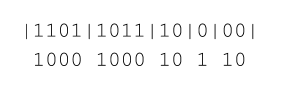
\includegraphics[width=0.4\textwidth]{images/obr_rank_select}}
\caption[Rank select usage in representation of sequence of elements with different size]{Rank select used in metadata, denoting start of the element.}
\label{obr:obr_rank_select}
\end{figure}


\section{Dynamic succinct data structures}

The most recent results in succinct data structures look into how to make these data structures more usable in real-life scenarios. Many times, the
strongest assumption of these data structures is, that the data we store is not changing in any way. For a few years now, there is a considerable effort put into dynamic succinct data structures. There are two types of what the word dynamic means. Let's say that our data structure represents some sequence of numbers. In some cases, it can refer to the ability to change some value in the underlying sequence. In other cases, it refers to the possibility to insert a new element at the arbitrary position in the sequence. Sometimes, it only means changing the element at an arbitrary position and adding the new element only at the end of the sequence.

\subsection{Searchable Partial Sums with Inserts}

\begin{theorem}
The Searchable Partial Sums with Inserts (SPSI) problem is asking for the data structure to
store sequence $x_1, x_2, \ldots , x_n$ of non-negative $l$-bits integers and supporting the opperations:
\begin{itemize}
    \item $sum(i) = \Sigma_{j=1}^{i} x_j$
    \item $search(s) = min(\{i : \Sigma_{j=1}{i} x_j > s \})$
    \item $update(i, k): \forall k \in Z, k \geq 0 \lor (k\leq 0 \implies x_i + k \geq 0): x_i \rightarrow x_i + k$
    \item $insert(i): x_1, x_2,\ldots, x_n \rightarrow x_1, x_2,\ldots , x_{i-1}, 0, x_{i}, \ldots , x_n$
\end{itemize}
\end{theorem}

This problem is also very popular in relation to succinct data structures. It is because of its close relationship with the bit-vectors.
As can be seen in [Dynamic], this data structure can be used to represent the bit-vector.

\section{Implementation}

In this work, we focus on transforming some of the ideas that were developed over years to real-life implementations. Many times, the solutions aiming at the best theoretical bounds are very complicated and build on top of several ideas from previous works. Many of the current best results from the perspective of theoretical complexity do not provide any implementation. We looked at what is the current status of working implementations and what theoretical bounds they reach.

We will now look at the best libraries that implement these succinct data structures. Libraries implementing succinct data structures are numerous and pretty common by now.

When we add the requirement of dynamism, we see that the number of libraries drops significantly. One of the most notable libraries supporting 
dynamic succinct data structures is DYNAMIC. It builds on top of the SPSI problem. Their implementation uses B-tree to represent this data structure. B-tree is a type of a $(a, b)$-tree, so we are free to choose the degree of a node in the tree and also the number of elements stored in one node. Using these two parameters, we can balance the implementation to get good tree depth and also ideal length of one node so it fits exactly into one cache line, making the implementation fast. Additionally, using the B-tree as an implementation for SPSI, DYNAMIC implements other succinct
data structures using their SPSI implementation. One of the main issues DYNAMIC implementat
